\section{Cauchy: Bringing Order to the Chaos of Calculus (1821)}

\subsection{From Intuition to Rigor: How Cauchy Rebuilt the Foundations of Calculus}

For centuries, mathematics operated on an unspoken assumption: **space is continuous, numbers behave, and infinite processes make sense**. From Eudoxus’ workaround for incommensurable numbers to Euclid’s seamless geometric world, continuity was treated as self-evident, not something that needed to be proven.  

Archimedes came closer than anyone to exposing the problem. His **method of exhaustion** let him approximate areas and volumes by stacking infinitely many smaller shapes, getting arbitrarily close to the true answer. But “arbitrarily close” isn’t the same as "equal to." He could show that the difference between his approximation and the real value shrank indefinitely, but he had no way of proving that it ever truly disappeared. It was an intuitive leap—a leap that worked, but one that nobody questioned.

And for nearly two thousand years, nobody had to.  

Then calculus happened.

By the 17th century, Newton and Leibniz revolutionized mathematics with their new language of motion and change. But they built it on **infinitesimals**—mysterious quantities that were "infinitely small" but never quite zero. These were useful for computations, but they were vague, lacking the kind of logical rigor that Euclid had once demanded of geometry. The ancient questions that had been swept under the rug by Eudoxus and Archimedes had returned in a new form.

Calculus worked. It produced astonishingly accurate results. But **why** did it work?  

By the early 19th century, this was no longer a question mathematicians could ignore. If calculus was going to be a reliable tool, it needed a firm logical foundation.

Augustin-Louis Cauchy saw this as a serious problem—and he had a solution.  

His approach? A new way of thinking about **limits, continuity, and density** that didn’t rely on vague infinitesimals but instead used sequences—real, well-defined numerical objects. He set out to do what no one had done before: define what it actually means for something to get "closer and closer" to a value, without assuming that the answer was self-evident.


\begin{tcolorbox}[
  colback=gray!5,
  colframe=black,
  title=\textbf{Historical Sidebar: Cauchy’s Catholic Calculus},
  fonttitle=\bfseries,
  width=\linewidth,
  enlarge left by=0mm,
  enlarge right by=0mm,
  boxrule=0.4pt,
  arc=2mm,
  left=4pt,
  right=4pt,
  top=6pt,
  bottom=6pt
]
Cauchy wasn’t just a mathematician—he was a militant Catholic in a post-Revolutionary France still wobbling between Enlightenment skepticism and monarchical restoration. And his mathematics reflected it.

\medskip

To Cauchy, ambiguity in analysis wasn’t merely a technical issue—it was a moral stain. The fuzziness of infinitesimals, the hand-waving arguments of early calculus? Spiritually suspect. Mathematics, like theology, was supposed to reflect eternal truths—and eternal truths don’t come with footnotes.

\medskip

His devout faith shaped his belief that truth must be absolute, unambiguous, and divinely ordered. So when he introduced rigorous definitions of limits, continuity, and convergence, it wasn’t just to clean up the field—it was an act of metaphysical hygiene. For Cauchy, a proof wasn’t valid unless it could stand before both God and a blackboard.

\medskip

\begin{center}
\emph{In Cauchy’s hands, calculus was not just precise—it was penitential.}
\end{center}
\end{tcolorbox}


\begin{figure}[H]
\centering
\begin{tikzpicture}[every node/.style={font=\footnotesize}]

% Panel 1
\comicpanel{0}{4}
  {Euclid}
  {Archimedes}
  {\textbf{Euclid:} Space is continuous. That’s just... obvious, right?}
  {(0,-0.5)}

% Panel 2
\comicpanel{6.5}{4}
  {Archimedes}
  {Euclid}
  {\textbf{Archimedes:} I can get as close as I want to the answer.  
That counts.}
  {(0,-0.5)}

% Panel 3
\comicpanel{0}{0}
  {Newton}
  {Leibniz}
  {\textbf{Newton:} Look, infinitesimals are totally real if you squint hard enough.}
  {(0,-0.5)}

% Panel 4
\comicpanel{6.5}{0}
  {Cauchy}
  {Everyone}
  {\textbf{Cauchy:} Cool story. Now define your terms or get out.}
  {(0,0.8)}

\end{tikzpicture}
\caption{Cauchy: dragging calculus from vibes to definitions, one sequence at a time.}
\end{figure}


\subsection{Cauchy’s Sequences: Getting Closer Without Ever Arriving}

To formalize limits, Cauchy turned to \textbf{sequences}—ordered lists of numbers approaching a particular value. He introduced what is now known as a \textbf{Cauchy sequence}, a sequence in which the terms become arbitrarily close to each other as the sequence progresses.  Here’s a simple, intuitive example:

\[
1,\ 1.5,\ 1.75,\ 1.875,\ 1.9375,\ 1.96875,\ \dots
\]

Each number in this sequence is halfway between the previous number and 2. So the terms keep creeping closer to 2—but they never quite get there.

More importantly, as the sequence goes on, the difference between consecutive terms shrinks:

\[
|1.5 - 1| = 0.5,\quad |1.75 - 1.5| = 0.25,\quad |1.875 - 1.75| = 0.125,\quad \dots
\]

Eventually, the terms are so close together that for any margin of error (say, $0.001$), there’s a point in the sequence beyond which all terms are within that tiny distance of each other. That’s the heart of a Cauchy sequence.

\textbf{It’s not about where the sequence is going—it’s about how tightly the terms huddle together as they go.}



This idea let Cauchy define what it means to approach a value: even in cases where the value itself might not be directly reachable.

Cauchy’s insight was that \textbf{if a sequence is converging to a real number, its terms must eventually stabilize and stop wandering off in different directions}. This concept was crucial because it provided a way to define limits without assuming the existence of infinitesimals.




\begin{figure}[H]
\centering
\begin{tikzpicture}[every node/.style={font=\footnotesize}]

% Panel 1: Student starts off confused about sequences
\comicpanel{0}{4}
  {Student}
  {Cauchy}
  {\textbf{Student:} So... if a sequence never reaches the limit, how does it "know" where it's going?}
  {(0,-0.5)}

% Panel 2: Cauchy sets the stage
\comicpanel{6.5}{4}
  {Student}
  {Cauchy}
  {\textbf{Cauchy:} It's not about reaching a destination. It's about the terms getting closer to each other.}
  {(0,-0.5)}

% Panel 3: Student begins to see the idea
\comicpanel{0}{0}
  {Student}
  {Cauchy}
  {\textbf{Student:} So you're saying if they stick close enough for long enough... that’s good enough?}
  {(0,0.8)}

% Panel 4: Cauchy, with a smirk
\comicpanel{6.5}{0}
  {Student}
  {Cauchy}
  {\textbf{Cauchy:} Yep. It's less “Where are we going?” and more “Are we huddled tight?”}
  {(0,0.8)}

\end{tikzpicture}
\caption{Cauchy’s big idea: a sequence doesn’t need to reach its limit — it just needs to get internally consistent.}
\end{figure}



\subsection{Defining Limits Without Infinitesimals}

\subsubsection{A Sequence-Based Illustration}

To make the concept of limits rigorous, Cauchy replaced the vague idea of “getting close” with something more precise: sequences.  Let’s begin with a concrete example. Consider the sequence:

\[
1,\ 1.5,\ 1.75,\ 1.875,\ 1.9375,\ 1.96875,\ \dots
\]

Each number in this sequence is halfway between the previous number and 2. The terms keep approaching 2—but never reach it.

Now notice: the terms get arbitrarily close to 2. That is, for any degree of closeness we care to specify (say, within \(0.001\)), we can find a point in the sequence beyond which all subsequent terms are within that distance of 2.

\textbf{This is how Cauchy defined a limit:} a number \( L \) is the limit of a sequence \( (a_n) \) if the terms of the sequence eventually get arbitrarily close to \( L \)—and stay close.

In modern notation, we would say:  
\[
\lim_{n \to \infty} a_n = L
\]
if the terms of \( a_n \) can be made as close to \( L \) as we like by taking \( n \) sufficiently large. Cauchy formalized this using sequences, not infinitesimals.

\begin{center}
\begin{tikzpicture}
    % Draw the horizontal axis
    \draw[->] (-1,0) -- (10,0) node[right] {\( n \)};
    
    % Draw the vertical axis
    \draw[->] (0,-1) -- (0,4) node[above] {\( a_n \)};
    
    % Limit L (horizontal dashed line)
    \draw[dashed] (-1,2.5) -- (10,2.5) node[right] {\( L \)};
    
    % Epsilon bands
    %\draw[dashed, red] (-1,3) -- (10,3) node[right] {\( L + \epsilon \)};
    %\draw[dashed, red] (-1,2) -- (10,2) node[right] {\( L - \epsilon \)};
    
    % Mark a threshold N
    %\draw[dotted, thick] (6,-0.2) -- (6,4) node[above] {\( N \)};
    
    % Plot sequence points
    \foreach \x/\y in {1/0.5, 2/1.5, 3/3, 4/2.8, 5/2.6, 6/2.55, 7/2.52, 8/2.51, 9/2.505} {
        \filldraw (\x,\y) circle (2pt);
    }
    
    % Labels for key points
    %\node[below] at (6,0) {\( N \)};
    \node[left] at (0,2.5) {\( L \)};
    
    % Text description
   % \node[right] at (7,1) {For \( n > N \), terms stay within \( \epsilon \) of \( L \)};
    
\end{tikzpicture}
\end{center}


\subsubsection{A Concrete Example: \( f(x) = 2x \)}

Suppose we want to understand what value \( f(x) = 2x \) approaches as \( x \) gets close to 3. In Cauchy’s framework, we consider a sequence of values getting closer and closer to 3.

Let’s define a sequence:

\[
x_n = 3 - \frac{1}{n}
\]

So \( x_1 = 2,\ x_2 = 2.5,\ x_3 = 2.666\dots \), and so on. Clearly, \( x_n \to 3 \) as \( n \to \infty \).

Now look at the corresponding values of the function:

\[
f(x_n) = 2x_n = 2 \left( 3 - \frac{1}{n} \right) = 6 - \frac{2}{n}
\]

As \( n \to \infty \), \( \frac{2}{n} \to 0 \), so:

\[
f(x_n) \to 6
\]

Therefore, Cauchy would say:

\[
\lim_{x \to 3} 2x = 6
\]

because for any sequence that approaches 3 (and doesn’t get stuck at 3), the values of \( f(x) = 2x \) along that sequence approach 6.


Cauchy made the idea of limits rigorous using sequences. By examining what happens to \( f(x) \) along sequences approaching a point, he gave analysis a foundation that replaced intuition with precision (without invoking infinitesimals).

\begin{figure}[H]
\centering
\begin{tikzpicture}[every node/.style={font=\footnotesize}, scale=1]

% Panel 1
\comicpanel{0}{4}
  {Student}
  {Mathematician}
  {\textbf{Student:} If we just keep getting closer and closer to a number... that counts as a limit, right?}
  {(0,-0.5)}

% Panel 2
\comicpanel{6.5}{4}
  {Mathematician}
  {Student}
  {\textbf{Mathematician:} Define “closer.”}
  {(0,-0.5)}

% Panel 3
\comicpanel{0}{0}
  {Mathematician}
  {Student}
  {\textbf{Mathematician:} We use epsilon. You pick how close.  
Then I prove we can always get there.}
  {(0,0.8)}

% Panel 4
\comicpanel{6.5}{0}
  {Student}
  {Mathematician}
  {\textbf{Student:} So… calculus is just high-precision stalking.}
  {(0,0.8)}

\end{tikzpicture}
\caption{Limits: for when intuition isn't clingy enough.}
\end{figure}






\subsection{Density: Filling in the Gaps}

\subsubsection{A Sequence-Based Illustration}


The idea of “filling in the gaps” goes way back. The Greeks were already grappling with it when they stumbled upon irrational numbers—quantities like \( \sqrt{2} \) that refused to be written as fractions. As we saw earlier, Eudoxus cleverly dodged the issue by comparing magnitudes instead of calculating them directly. But even then, there was a lurking question:

\begin{quote}
Are the rational numbers enough to describe the number line?
\end{quote}

For a while, it looked like yes. Rational numbers seemed to be everywhere. No matter how small a gap you chose, there was always another rational number inside it. But Cauchy’s work on sequences revealed something subtle: while rational numbers can get arbitrarily close to any point on the line, they sometimes \textit{never actually reach} their destination.

Let’s take a concrete example:

\[
1.4,\ 1.41,\ 1.414,\ 1.4142,\ 1.41421,\ \dots
\]

This sequence seems to be converging to \( \sqrt{2} \). And yet, every number in the list is rational. Try as you might, you’ll never land on \( \sqrt{2} \) using fractions alone. The terms are good approximations, but the true limit—the thing they’re chasing—is just out of reach.

This is where the idea of \textbf{density} comes in.

A set \( S \subset \mathbb{R} \) is said to be \textbf{dense} in \( \mathbb{R} \) if, for any two real numbers \( a \) and \( b \) with \( a < b \), there exists an element \( x \in S \) such that:

\[
a < x < b
\]

In plain terms: between any two real numbers—no matter how small the gap—there’s always at least one member of \( S \) inside it.


% Optional: remove if too modern, but adapted to match sequence logic
\begin{center}
\begin{tikzpicture}
    % Draw the horizontal axis
    \draw[->] (-1,0) -- (10,0) node[right] {\( n \)};
    
    % Draw the vertical axis
    \draw[->] (0,-1) -- (0,4) node[above] {\( a_n \)};
    
    % Limit L (horizontal dashed line)
    \draw[dashed] (-1,2.5) -- (10,2.5) node[right] {\( L \)};
    
    % Plot sequence points before N
    \foreach \x/\y in {1/0.5, 2/1.2, 3/3.5, 4/2.8} {
        \filldraw[blue] (\x,\y) circle (2pt);
    }
    
    % Plot sequence points after N (converging to L)
    \foreach \x/\y in {6/2.6, 7/2.55, 8/2.52, 9/2.51, 10/2.505} {
        \filldraw[green] (\x,\y) circle (2pt);
    }
    
    % Mark a threshold N
    \draw[dotted, thick] (5,-0.2) -- (5,4) node[above] {\( N \)};
    
    % Labels for key points
    \node[below] at (5,0) {\( N \)};
    \node[left] at (0,2.5) {\( L \)};
    
    % Text description
    \node[align=left, right] at (7,1) {For large \( n \),\\ \( a_n \to L \)};
    
\end{tikzpicture}
\end{center}



But Cauchy's insight went further: he considered sequences made entirely of rational numbers, like the example above, that converge toward a real number that is \textit{not} rational. Such sequences reveal that although rational numbers are densely packed, they don’t capture every possible limit.

\subsubsection{Concrete Examples}

\begin{itemize}
    \item \textbf{Rational numbers \( \mathbb{Q} \)} are dense in \( \mathbb{R} \).
    \begin{itemize}
        \item Between 1.41 and 1.42? Try \( \frac{1415}{1000} = 1.415 \)
        \item Between \( \pi \) and \( \pi + 0.00001 \)? There’s a rational in there too.
    \end{itemize}

    \item \textbf{Integers \( \mathbb{Z} \)} are \textbf{not} dense in \( \mathbb{R} \).
    \begin{itemize}
        \item There’s nothing between 2 and 3 in \( \mathbb{Z} \).
    \end{itemize}

    \item \textbf{Irrational numbers} are also dense in \( \mathbb{R} \).
    \begin{itemize}
        \item Example: Between \( \frac{1}{2} \) and \( \frac{3}{4} \), try \( \frac{5}{8} + \frac{\sqrt{2}}{1000} \)
    \end{itemize}
\end{itemize}


\textbf{But here’s the problem:} While rational numbers are dense, they aren’t \textbf{complete}. That sequence converging to \( \sqrt{2} \)? It never actually reaches it—not because it fails to get close, but because the destination isn’t even in the set.

This led to a fundamental insight: \textbf{being dense doesn’t mean you’ve filled all the gaps.} Cauchy’s sequences exposed the flaw. To fix it, mathematicians had to expand their view—constructing the real numbers \( \mathbb{R} \) as a completion of the rationals using those very sequences.

In other words: \textbf{density covers ground, but completeness builds the road.}




\begin{figure}[H]
\centering
\begin{tikzpicture}[every node/.style={font=\footnotesize}]

% Panel 1
\comicpanel{0}{4}
  {Analyst}
  {Student}
  {\textbf{Analyst:} Rational numbers are dense. No matter where you zoom in, there’s always another one.}
  {(0,-0.5)}

% Panel 2
\comicpanel{6.5}{4}
  {Student}
  {Analyst}
  {\textbf{Student:} But if they’re everywhere... how come I still can’t land on $\sqrt{2}$?}
  {(0,-0.5)}

% Panel 3
\comicpanel{0}{0}
  {Analyst}
  {Student}
  {\textbf{Analyst:} Density just fills the gaps. It doesn’t guarantee the destination actually exists.}
  {(0,0.8)}

% Panel 4
\comicpanel{6.5}{0}
  {Student}
  {Analyst}
  {\textbf{Student:} So the rationals are like a crowd with no house to go to. Got it.}
  {(0,0.8)}

\end{tikzpicture}
\caption{Dense but not complete: The rationals are everywhere, except where it counts.}
\end{figure}




\subsection{Continuity: Making Functions Behave}

\subsubsection{A Sequence-Based Illustration}


Before Cauchy, continuity was more of a geometric idea: if you could draw a function’s graph without lifting your pencil, it was “continuous.” But this was vague and not useful for analysis. Cauchy changed that by giving continuity a precise, sequence-based definition.

Let’s begin with a simple, intuitive example.


Consider the function \( f(x) = x^2 \). Suppose we’re interested in whether this function is continuous at \( x = 2 \). Try plugging in a sequence of values that get closer to 2:

\[
1.5,\ 1.9,\ 1.99,\ 2.01,\ 2.1,\ 2.5,\ \dots
\]

Evaluating \( f(x) = x^2 \) at those points gives:

\[
2.25,\ 3.61,\ 3.9601,\ 4.0401,\ 4.41,\ 6.25,\ \dots
\]

As \( x \to 2 \), the function values get arbitrarily close to 4. That’s what we expect from a continuous function: \textbf{inputs near 2 produce outputs near \( f(2) = 4 \)}.

\subsubsection{The Formal Definition via Sequences}

A function \( f(x) \) is \textbf{continuous at a point \( c \)} if for every sequence \( (x_n) \) that converges to \( c \), the sequence \( f(x_n) \) converges to \( f(c) \).

In symbols:

\[
\text{If } x_n \to c, \text{ then } f(x_n) \to f(c)
\]

This captures the intuitive idea that when inputs approach \( c \), their outputs should approach \( f(c) \). If this happens for \textit{every} sequence that approaches \( c \), then the function is continuous at \( c \).

\begin{center}
\begin{tikzpicture}
    % Draw x and y axes
    \draw[->] (-1,0) -- (7,0) node[right] {\( x \)};
    \draw[->] (0,-1) -- (0,5) node[above] {\( f(x) \)};
    
    % Function curve
    \draw[thick, blue, domain=0.5:6.5, smooth] plot (\x, {0.3*\x*\x - 0.8*\x + 2});
    
    % Mark c on x-axis
    \draw[dashed] (3,0) -- (3,2.8);
    \filldraw[black] (3,0) circle (2pt) node[below] {\( c \)};
    
    % Mark f(c) on y-axis
    \draw[dashed] (0,2.8) -- (3,2.8);
    \filldraw[black] (0,2.8) circle (2pt) node[left] {\( f(c) \)};
    
    % Sequence points approaching c from left and right
    \foreach \x/\y in {2.5/2.125, 2.7/2.47, 2.9/2.755, 3.1/2.845, 3.3/3.01, 3.5/3.125} {
        \filldraw[green] (\x,\y) circle (2pt);
    }
    
    % Plot point on curve at (c, f(c))
    \filldraw[black] (3,2.8) circle (2pt);
    
    % Labels and explanation
    \node[align=left, right] at (5,4) {Sequences approaching \( c \) \\ result in outputs approaching \( f(c) \)};
\end{tikzpicture}
\end{center}

\subsubsection{Concrete Examples}

\begin{itemize}
    \item \textbf{Continuous: \( f(x) = x^2 \) at \( x = 2 \)}  
    Let \( x_n \to 2 \). Then \( f(x_n) = x_n^2 \to 4 = f(2) \). So the function is continuous at 2.

    \item \textbf{Continuous: \( f(x) = \sin x \)}  
    For any sequence \( x_n \to c \), we know \( \sin x_n \to \sin c \). So \( f(x) = \sin x \) is continuous everywhere.

    \item \textbf{Not Continuous: Jump Discontinuity}  
    Define:
    \[
    f(x) = \begin{cases}
      1 & \text{if } x < 0 \\
      2 & \text{if } x \geq 0
    \end{cases}
    \]
    Consider the sequence \( x_n = -\frac{1}{n} \to 0 \). Then \( f(x_n) = 1 \), but \( f(0) = 2 \). Since \( f(x_n) \not\to f(0) \), the function is \textbf{not} continuous at \( x = 0 \).
\end{itemize}


\textbf{Conclusion:} Cauchy’s definition of continuity using sequences replaced vague geometric intuition with precise behavior: if getting closer to a point with inputs always brings the outputs closer to the function value at that point, the function is continuous there.


\begin{center}
\begin{figure}[H]
\centering
\begin{tikzpicture}[every node/.style={font=\small}]

% Panel 1 — Stick figure introduces the old idea
\comicpanel{0}{4}
  {Historian}
  {Analyst}
  {\textbf{Historian:} A function is continuous if you can draw it without lifting your pen.}
  {(0,-0.6)}

% Panel 2 — Analyst introduces Cauchy’s idea
\comicpanel{7}{4}
  {Historian}
  {Analyst}
  {\textbf{Analyst:} Actually, Cauchy defined it using $\varepsilon$ and $\delta$. It’s... more intense.}
  {(0,-0.6)}

% Panel 3 — Historian confused
\comicpanel{0}{0}
  {Historian}
  {Analyst}
  {\textbf{Historian:} What do you mean “for every $\varepsilon$ there exists a $\delta$”? That sounds like a threat.}
  {(0,0.6)}

% Panel 4 — Analyst finishes them off
\comicpanel{7}{0}
  {Historian}
  {Analyst}
  {\textbf{Analyst:} Continuity is just when no matter how tight the margin, you can squeeze the function into it. Like… with math tweezers.}
  {(0,0.6)}

\end{tikzpicture}
\caption{Cauchy's epsilon-delta definition of continuity: the part where analysis gets real.}
\end{figure}
\end{center}






\subsection{Cauchy’s Definition of Differentiability}

\subsubsection{A Sequence-Based Illustration}

Before Cauchy, differentiation was mostly an intuitive process—a way to talk about how quantities change instantly. But what exactly does “instantaneous change” mean?

Cauchy gave the first rigorous answer using the language of sequences and limits.


Let’s take the function \( f(x) = x^2 \), and consider how the value of the difference quotient behaves near \( x = 3 \).

Try plugging in a sequence of small values for \( h \) approaching zero:

\[
h = 1,\ 0.5,\ 0.1,\ 0.01,\ 0.001,\ \dots
\]

Now compute the difference quotient:

\[
\frac{f(3 + h) - f(3)}{h} = \frac{(3 + h)^2 - 9}{h}
= \frac{9 + 6h + h^2 - 9}{h} = \frac{6h + h^2}{h} = 6 + h
\]

As \( h \to 0 \), this expression approaches 6. In other words, the outputs of the difference quotient sequence converge to a single value.

\textbf{That’s the idea:} If, for every sequence \( h_n \to 0 \), the sequence of difference quotients

\[
\frac{f(c + h_n) - f(c)}{h_n}
\]

converges to the same number, then the function is differentiable at \( c \), and that number is the derivative.

\subsubsection{The Formal Definition via Sequences}

A function \( f(x) \) is said to be \textbf{differentiable at a point \( c \)} if, for every sequence \( (h_n) \) with \( h_n \to 0 \) and \( h_n \neq 0 \), the sequence

\[
\frac{f(c + h_n) - f(c)}{h_n}
\]

converges to a fixed real number. That number is called the derivative of \( f \) at \( c \), written \( f'(c) \).

\begin{center}
\begin{tikzpicture}
    % Draw axes
    \draw[->] (-1,0) -- (7,0) node[right] {\( x \)};
    \draw[->] (0,-1) -- (0,5) node[above] {\( f(x) \)};
    
    % Function curve
    \draw[thick, blue, domain=0.5:6.5, smooth] plot (\x, {0.2*\x*\x - 0.5*\x + 2});
    
    % Points on the curve
    \filldraw[black] (3,2.5) circle (2pt) node[above left] {\( (c, f(c)) \)};
    \filldraw[black] (5,3.1) circle (2pt) node[above right] {\( (c+h, f(c+h)) \)};
    
    % Secant line
    \draw[dashed, red] (3,2.5) -- (5,3.1);
    \node[right] at (4,3) {\footnotesize Secant line};
    
    % Tangent line at c
    \draw[dashed, green] (1,1.7) -- (6,3.4);
    \node[left] at (1,1.7) {\footnotesize Tangent line (as \( h_n \to 0 \))};
    
    % Vertical lines showing f(c) and f(c+h)
    \draw[dotted] (3,0) -- (3,2.5);
    \draw[dotted] (5,0) -- (5,3.1);
    
    % Horizontal distance h
    \draw[<->] (3,-0.5) -- (5,-0.5);
    \node[below] at (4,-0.5) {\( h \)};
    
    % Difference quotient representation
    \draw[<->] (5.3,2.5) -- (5.3,3.1);
    \node[right] at (5.3,2.8) {\( f(c+h) - f(c) \)};
\end{tikzpicture}
\end{center}

\subsubsection{Examples}

\textbf{Differentiable: \( f(x) = \ln(x) \) at \( x = 1 \)}  

Let \( h_n \to 0 \), with \( h_n \neq 0 \). Then:

\[
\frac{f(1 + h_n) - f(1)}{h_n} = \frac{\ln(1 + h_n)}{h_n} \to 1
\]

So the function is differentiable at \( x = 1 \) with derivative \( f'(1) = 1 \).

\begin{figure}[H]
\centering
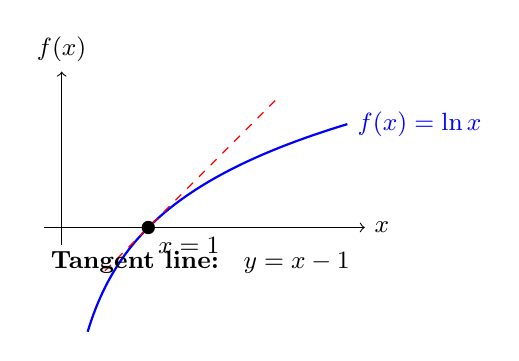
\begin{tikzpicture}[scale=1.1, every node/.style={font=\small}]

  % Axes
  \draw[->] (-0.2,0) -- (3.5,0) node[right] {\(x\)};
  \draw[->] (0,-0.2) -- (0,1.8) node[above] {\(f(x)\)};

  % Function curve: f(x) = ln(x)
  \draw[thick, blue, domain=0.3:3.3, samples=100] plot (\x, {ln(\x)}) node[right] {\(f(x) = \ln x\)};

  % Tangent line at x = 1: slope = 1 → y = x - 1
  \draw[dashed, red, domain=0.5:2.5] plot (\x, {\x - 1});

  % Point of tangency
  \filldraw[black] (1,0) circle (2pt) node[below right] {\(x = 1\)};

  % Label
  \node at (1.6,-0.4) {\textbf{Tangent line: } \(y = x - 1\)};
\end{tikzpicture}
\caption{The function \( f(x) = \ln(x) \) is differentiable at \( x = 1 \). The tangent line at that point has slope 1, which is the limit of the difference quotient as \( h_n \to 0 \).}
\end{figure}










\textbf{Differentiable: \( f(x) = \sin x \) at any \( x \)}  

    For any sequence \( h_n \to 0 \), the difference quotient:

    \[
    \frac{\sin(x + h_n) - \sin(x)}{h_n}
    \]

    converges to \( \cos(x) \). So sine is differentiable everywhere.
    
    





\begin{figure}[H]
\centering
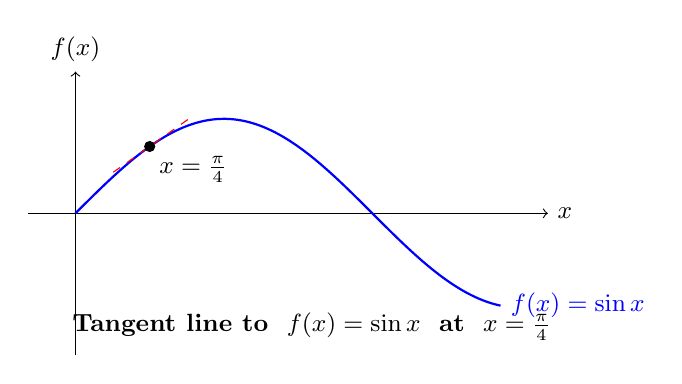
\begin{tikzpicture}[scale=1.2, every node/.style={font=\small}]
  % Axes
  \draw[->] (-0.5,0) -- (5,0) node[right] {\(x\)};
  \draw[->] (0,-1.5) -- (0,1.5) node[above] {\(f(x)\)};

  % Sine curve
  \draw[thick, blue, domain=0:4.5, samples=100] plot (\x, {sin(deg(\x))}) node[right] {\(f(x) = \sin x\)};

  % Tangent line at x = pi/4 ≈ 0.785 (cos(pi/4) = sqrt(2)/2 ≈ 0.707)
  % Line: y = cos(pi/4)(x - pi/4) + sin(pi/4)
  \draw[dashed, red, domain=0.4:1.2] 
    plot (\x, {0.7071*(\x - 0.7854) + 0.7071});

  % Point of tangency
  \filldraw[black] (0.7854,0.7071) circle (1.5pt);
  \node[below right] at (0.7854,0.7071) {\(x = \frac{\pi}{4}\)};

  % Label
  \node at (2.5,-1.2) {\textbf{Tangent line to } \( f(x) = \sin x \) \textbf{ at } \( x = \frac{\pi}{4} \)};
\end{tikzpicture}
\caption{
The sine function is differentiable at \( x = \frac{\pi}{4} \). The tangent line at this point has slope \( \cos\left(\frac{\pi}{4}\right) = \frac{\sqrt{2}}{2} \), which is the limit of the difference quotient as \( h_n \to 0 \).
}
\end{figure}
    
    
  

\textbf{Not Differentiable: \( f(x) = |x| \) at \( x = 0 \)}  

    Let \( h_n \to 0 \), and consider two cases:

    \begin{itemize}
        \item If \( h_n > 0 \), then \( \frac{|h_n|}{h_n} = 1 \)
        \item If \( h_n < 0 \), then \( \frac{|h_n|}{h_n} = -1 \)
    \end{itemize}

    Since the values of the difference quotient depend on the direction \( h_n \) approaches zero, and do not converge to a single number, \( f(x) = |x| \) is \textbf{not} differentiable at 0.




\begin{figure}[H]
\centering
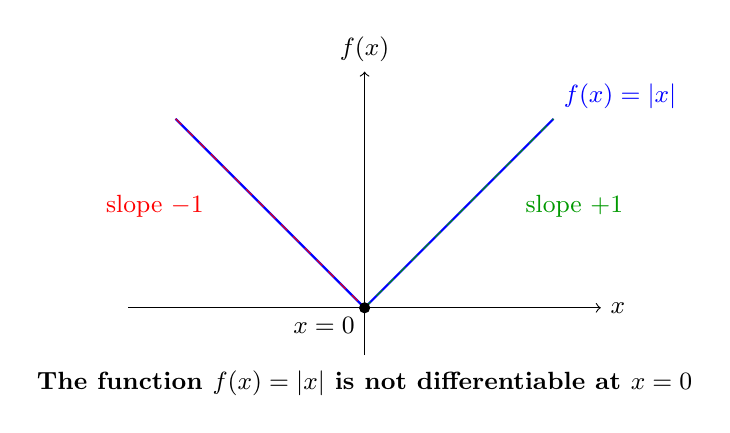
\begin{tikzpicture}[scale=1.2, every node/.style={font=\small}]

  % Axes
  \draw[->] (-2.5,0) -- (2.5,0) node[right] {\(x\)};
  \draw[->] (0,-0.5) -- (0,2.5) node[above] {\(f(x)\)};

  % Absolute value function
  \draw[thick, blue, domain=-2:2] plot (\x, {abs(\x)}) node[above right] {\(f(x) = |x|\)};

  % Secant lines approaching from the left and right
  \draw[dashed, red] (-2,2) -- (0,0);
  \draw[dashed, green!60!black] (0,0) -- (2,2);

  % Mark the corner
  \filldraw[black] (0,0) circle (1.5pt);
  \node[below left] at (0,0) {\(x = 0\)};

  % Labels for secants
  \node[red, below left] at (-1.6,1.3) {\small slope \(-1\)};
  \node[green!60!black, below right] at (1.6,1.3) {\small slope \(+1\)};

  % Description
  \node at (0,-0.8) {\textbf{The function \( f(x) = |x| \) is not differentiable at \( x = 0 \)}};

\end{tikzpicture}
\caption{
The left-hand and right-hand difference quotients of \( f(x) = |x| \) approach different values as \( x \to 0 \). From the left, the slope is \(-1\); from the right, it’s \(+1\). Since the limit does not exist, \( f \) is not differentiable at 0.
}
\end{figure}






\textbf{Conclusion:} Cauchy’s definition of the derivative made instantaneous change precise. If all sequences of small increments produce the same limiting slope, the function is differentiable at that point. With this, calculus gained a rigorous foundation rooted in sequence-based reasoning.


\begin{tcolorbox}[
  colback=gray!5,
  colframe=black,
  title=\textbf{Historical Sidebar: Cauchy vs. the Revolution},
  fonttitle=\bfseries,
  width=\linewidth,
  enlarge left by=0mm,
  enlarge right by=0mm,
  boxrule=0.4pt,
  arc=2mm,
  left=4pt,
  right=4pt,
  top=6pt,
  bottom=6pt
]
Cauchy wasn’t just a devout Catholic—he was a die-hard royalist who openly supported the Bourbon monarchy and loathed the ideals of the French Revolution. In a time when liberalism, secularism, and abstraction were sweeping through the intellectual elite, Cauchy stood on the opposite shore, building walls instead of bridges.

\medskip

His mathematics reflected that ideology. Where others were embracing flexibility, generality, and creative looseness, Cauchy insisted on structure, clarity, and absolute rigor. To him, mathematical vagueness wasn’t a style choice: it was a moral failure. And that did not make him popular in post-Revolutionary France.

\medskip

Academics around him found his tone grating, his piety rigid, and his insistence on moral discipline out of step with the era’s spirit of intellectual rebellion. While they sought freedom in abstraction, Cauchy was restoring order.

\medskip

\begin{center}
\emph{Where the Enlightenment sought liberty, Cauchy offered penance.}
\end{center}
\end{tcolorbox}

\begin{figure}[H]
\centering
\begin{tikzpicture}[every node/.style={font=\small}]

% Panel 1 — Stick figure introduces the old idea
\comicpanel{0}{4}
  {Historian}
  {Analyst}
  {\textbf{Historian:} Derivatives are just slopes. You draw a tangent line and boom—done.}
  {(0,-0.6)}

% Panel 2 — Analyst introduces Cauchy’s idea
\comicpanel{7}{4}
  {Historian}
  {Analyst}
  {\textbf{Analyst:} Actually, Cauchy defined the derivative as a limit of a difference quotient.}
  {(0,-0.6)}

% Panel 3 — Historian confused
\comicpanel{0}{0}
  {Historian}
  {Analyst}
  {\textbf{Historian:} So we’re just supposed to watch $h$ get smaller and hope the whole thing doesn’t explode?}
  {(0,0.6)}

% Panel 4 — Analyst finishes them off
\comicpanel{7}{0}
  {Historian}
  {Analyst}
  {\textbf{Analyst:} If the limit exists, you get a derivative. If it doesn’t, you get an existential crisis.}
  {(0,0.6)}

\end{tikzpicture}
\caption{Cauchy's definition of differentiability: limits, slopes, and the edge of sanity.}
\end{figure}


\subsection{The Aftermath: Cauchy vs. Everyone}

Cauchy revolutionized calculus. He took mushy metaphors and turned them into machinery. He transformed squishy ideas into sequenced rigor. He kicked out infinitesimals like a bouncer at a logic nightclub.

And what did he get for it?

Exiled. Overlooked. Filed under “too intense, too early.”

Cauchy was right—but he was right at the wrong time. A legitimist monarchist in post-revolutionary France, a devout Catholic in a secularizing academy, and (perhaps most offensively of all) a man who insisted on $\varepsilon$–$\delta$ proofs when everyone else just wanted to draw curves and vibe.

He refused to swear allegiance to the July Monarchy, lost his teaching posts, and spent years tutoring royal exiles instead of shaping the mathematical canon in Paris. His contemporaries shrugged at his rigor. It wasn’t until Weierstrass and friends came along decades later that people dusted off Cauchy’s notebooks and realized, “Oh. He solved it.”

Let’s recap what Cauchy actually did—because it’s a lot.

\begin{center}
\renewcommand{\arraystretch}{1.4}
\begin{tabular}{|p{3.5cm}|p{5cm}|p{5cm}|}
\hline
\textbf{Concept} & \textbf{Before Cauchy} & \textbf{Cauchy’s Redefinition} \\
\hline
\textbf{Limits} & “Getting close” meant... vibes. & Defined rigorously using sequences and convergence criteria. \\
\hline
\textbf{Continuity} & “Draw it without lifting your pen.” & If $x_n \to c$, then $f(x_n) \to f(c)$ for every sequence. \\
\hline
\textbf{Differentiation} & Slopes of tangents—when the picture was nice. & Limit of difference quotients via sequences: $\displaystyle \lim_{h_n \to 0} \frac{f(c + h_n) - f(c)}{h_n}$. \\
\hline
\textbf{Density} & Rational numbers seemed to cover everything. & Showed rationals are dense but not complete—limits of rational sequences may be irrational. \\
\hline
\end{tabular}
\end{center}


\textbf{Bottom line:}  
Cauchy gave us a version of calculus that didn’t depend on magical infinitesimals or geometric intuition. He replaced hand-waving with precision—and got banished for his trouble.

\begin{itemize}
  \item Define limits rigorously? \checkmark
  \item Refuse to bend the knee to a monarchy? \checkmark
  \item Get iced out of academic prestige while Europe uses your math in secret? \checkmark\checkmark
\end{itemize}

Cauchy didn’t just change the rules. He \textit{wrote} them. But history stamped his paper “revised by others” and filed it under “rediscovered later.”





\begin{tcolorbox}[colback=blue!5!white, colframe=blue!50!black, 
  title={Historical Sidebar: The July Monarchy—When France Hit “Reboot” on Royalty}]
  
      The \textbf{July Monarchy} (1830–1848) was France’s post-revolutionary, mid-chaos, semi-bourgeois experiment in constitutional monarchy. It began when the ultra-royalist Charles X was kicked out after trying to turn back the clock to divine-right absolutism. In his place, the more moderate \textbf{Louis-Philippe} became “King of the French” (not “King of France”—branding matters), promising to respect the Charter of 1830 and pretend that popular sovereignty was cool now.
  
      \medskip
  
      In reality, the July Monarchy was a weird political chimera: part monarchy, part liberal republic, mostly confused. It catered to the bourgeois elite, tried to keep revolutionaries and royalists both at arm’s length, and failed to make anyone truly happy. The working class saw no real progress, intellectuals chafed under censorship, and legitimists (like \textbf{Cauchy}) refused to swear allegiance on principle.
  
      \medskip
  
      Cauchy’s refusal to endorse the regime cost him his Paris professorship. He spent much of the 1830s tutoring exiled royals in places like Turin and Prague. While France half-heartedly modernized under Louis-Philippe’s reign, Cauchy quietly redefined calculus in exile. It wouldn’t be the first time French politics got in the way of good math.
  
      \medskip
  
      In 1848, after years of protests and a few more bad decisions, the July Monarchy collapsed in yet another revolution. Louis-Philippe abdicated and fled to England disguised as “Mr. Smith.” Seriously.
  
      \medskip
  
      \textbf{Fun fact:} The July Monarchy is often remembered as the regime of “order without justice, and reform without progress.” Cauchy might’ve added: “And tenure without rigor.”
  
\end{tcolorbox}

\begin{figure}[H]
\centering
\begin{tikzpicture}[every node/.style={font=\small}]

% Panel 1
\comicpanel{0}{4}
  {Cauchy}
  {Academia}
  {\textbf{Cauchy:} I rewrote the foundations of calculus using sequences and rigorous limits.}
  {(0,-0.6)}

% Panel 2
\comicpanel{7}{4}
  {Academia}
  {Cauchy}
  {\textbf{Academia:} Fascinating. Now please swear allegiance to the king we actually like.}
  {(0,-0.6)}

% Panel 3
\comicpanel{0}{0}
  {Cauchy}
  {Academia}
  {\textbf{Cauchy:} No. But here's a paper proving the rationals are incomplete.}
  {(0,0.6)}

% Panel 4
\comicpanel{7}{0}
  {Academia}
  {Cauchy}
  {\textbf{Academia:} Enjoy Switzerland. We'll rediscover your work in 50 years.}
  {(0,0.6)}

\end{tikzpicture}
\caption{Cauchy: too rigorous, too royalist, too early.}
\end{figure}
